\section{Security Use Cases}
\label{sec:threat_model}

Building on the adversary model defined in Section~\ref{subsec:threat_model}, this section analyzes the detection guarantees provided by each component and illustrates the end-to-end security pipeline through operational use cases. This analysis validates the closed-loop enforcement cycle introduced in Section~\ref{subsec:defense_concept}: detect, reach consensus, update scores, filter, and deter. On the consensus plane, we additionally assume $\mathcal{A}$ controls up to $f < n/3$ RPKI-enabled nodes with bounded computation and adaptive corruption subject to $\Delta_{corrupt} > T_{window}$. Under this model, the PoP consensus mechanism provides four guarantees: (1)~\emph{Sybil resistance} through mandatory RPKI certificate verification; (2)~\emph{consensus safety} via deterministic hash-based creator selection and the $2f{+}1$ signature requirement; (3)~\emph{liveness} within $T_{window} + R \cdot T_{block} + \Delta$ under partial synchrony; and (4)~\emph{incentive compatibility} with a $6.5\times$ honest-to-dishonest earning differential. Formal proofs appear in Appendix~\ref{app:security_proofs}.


\subsection{Experimental Setup}
\label{subsec:detection_guarantees}

The attack detection and enforcement pipeline operates in four sequential phases. In Phase~1 (\emph{Observe}), each RPKI-enabled AS monitors BGP announcements received from its non-RPKI neighbors through four independent detectors. In Phase~2 (\emph{Detect}), when any detector flags an anomaly, the observer creates a transaction containing the BGP observation details, the attack classification, and the predetermined penalty amount. In Phase~3 (\emph{Consensus}), the transaction is broadcast to all RPKI validators, who independently verify the claim and provide endorsement signatures within the 30-second competition window; consensus is reached when the signature count meets the PoP threshold ($\tau = \max(3, \min(\lfloor N/3 \rfloor + 1, 5))$). In Phase~4 (\emph{Record}), the consensus-confirmed transaction is committed to the blockchain as an immutable record.

Table~\ref{tab:attack_detection_mechanisms} summarizes the detection method, graduated penalty schedule, and performance targets for each attack type. All four types share an escalating penalty structure: first offense incurs an attack-specific penalty (10--25 points depending on severity), repeated attacks within 30 days add a 30-point penalty, and persistent attackers (3+ total) receive an additional 50-point penalty.

\begin{table}[t]
\centering
\caption{Attack Detection: Methods, Penalties, and Targets}
\label{tab:attack_detection_mechanisms}
\setlength{\tabcolsep}{5pt}
\begin{tabular}{lllcc}
\toprule
\textbf{Attack Type} & \textbf{Detector} & \textbf{1st Penalty} & \textbf{Target} & \textbf{Response} \\
\midrule
Prefix Hijack    & ROA mismatch  & $-$20\,pts & $>$95\% & $<$10\,s \\
Subprefix Hijack & Hierarchical  & $-$18\,pts & $>$92\% & $<$20\,s \\
Route Flapping   & Temporal      & $-$10\,pts & $>$94\% & $<$60\,s \\
Bogon Injection  & Bogon DB      & $-$25\,pts & $>$99\% & $<$\,2\,s \\
\bottomrule
\end{tabular}
\end{table}

We now argue the correctness of each detector under the adversary model above.

\BfPara{Prefix hijack}
Detection is complete for ROA-covered prefixes: every incoming announcement is checked against the full ROA database, and any origin AS mismatch is flagged. False negatives are impossible for prefixes with valid ROA entries, since the check is a deterministic comparison.

\BfPara{Subprefix hijack}
A more-specific announcement whose origin differs from the covering ROA entry is unauthorized by construction. The hierarchical detector traverses the ROA prefix tree, ensuring that no more-specific route can bypass detection as long as the parent prefix has a valid ROA.

\BfPara{Bogon injection}
IANA reserved ranges (RFC~1918, RFC~5737, RFC~6598) are definitionally illegitimate in the global routing table. No legitimate AS should originate them, yielding zero false negatives by definition and near-zero false positives (only misconfigured routers leaking private space).

\BfPara{Route flapping}
The temporal detector applies a configurable threshold (default: 5 announcements in 60 seconds). Unlike the other three detectors, this is a heuristic with a known precision trade-off: legitimate route instability during convergence events can trigger false positives. Operators can tune \texttt{FLAP\_THRESHOLD} to balance sensitivity against false-positive rates for their environment.Finally, the conclusive route flapping decision is produced by postdoc analyses trough longitudinal study.

\BfPara{Collusion resistance}
The PoP consensus threshold is capped at 5 signatures ($\tau = \max(3, \min(\lfloor N/3 \rfloor + 1, 5))$), raising the question of whether 5 colluding RPKI observers could frame an innocent non-RPKI AS. Three mechanisms mitigate this risk. First, observer discovery (Algorithm~\ref{alg:observer_discovery}) selects validators based on AS-path proximity, so colluding nodes must be topologically adjacent to the target, a constraint that limits the attacker's reach. Second, the false accusation penalty ($-20$ BGPCOIN per rejected attack proposal, Algorithm~\ref{alg:create_transaction}) makes sustained false reporting economically costly: an attacker drains its coin balance after a small number of failed accusations. Third, the blockchain's immutable audit trail enables post-hoc cross-validation audits (Appendix~\ref{app:security_proofs}) that can retrospectively identify systematic bias in an observer's reports, triggering accuracy multiplier reduction and coin slashing. While these mechanisms raise the bar for collusion, we acknowledge that a coordinated supermajority attack ($f \geq n/3$) remains outside our threat model and represents an important direction for future work.

Beyond the four evaluated attack types, BGP-Sentry's architecture supports detection of additional BGP threats. Table~\ref{tab:other_attacks} summarizes extensible attack types and the system components that would address them. Comprehensive evaluation of these types remains future work.




% =======================
% Attack Detection and Reputation-based Deterrence Effectiveness
% Validates BGP Observation Layer, Trust Engines, and Trust Score mechanisms
% Demonstrates integrated architectural coordination and behavioral modification
% =======================
\subsection{Attack Detection and Reputation-based Deterrence Effectiveness}
\label{subsec:attack_detection_effectiveness}

BGP-Sentry achieved high recall across all network scales: 75\% at 100 ASes (3 of 4 ground truth attacks detected) and 100\% at 200, 500, and 1{,}000 ASes (all 4 attack patterns detected). {\color{red}At 1{,}000 ASes, the system achieved perfect precision (1.0), recall (1.0), and F1 score (1.0) with zero false positives.} Precision at smaller scales was lower (6.8--9.5\%) due to false positives from the route flapping detector on frequently-announced legitimate prefixes---a tunable trade-off controlled by the FLAP\_THRESHOLD parameter. The system processed 7,069 to 80,665 observations per run, writing 4,581 to 6,558 blocks to the blockchain with verified SHA-256 hash chain and Merkle root integrity across all experiments.

Each attack type validates different architectural layer combinations, demonstrating comprehensive integration effectiveness. Prefix hijacking validates BGP Observation Layer + Reactive Trust Engine coordination, while route flapping validates Adaptive Trust Engine real-time analysis capabilities.

Figure~\ref{fig:per_attack_metrics} presents per-attack-type detection performance: prefix hijacking, subprefix hijacking, and bogon injection achieve near-perfect precision and recall, while route flapping trades precision for high sensitivity---a configurable parameter via \texttt{FLAP\_THRESHOLD}. The confusion matrix confirms zero cross-type misclassification; the only errors are flapping false positives on legitimate prefixes.



The trust scoring system achieved substantial behavioral modification across all categories. Non-RPKI ASes that originated attacks saw their trust scores drop from the initial 50 (Neutral) to the Suspicious range (30--49), while ASes with only legitimate announcements maintained Neutral or higher scores. As trust scores decline, non-RPKI ASes experience gradual loss of network acceptability, incentivizing improved routing behavior.


% Per-attack detection performance (representative: caida_200)
% TODO: Replace demo data with real caida_200 experimental results
\begin{figure}[t]
\centering
\begin{tikzpicture}
\begin{axis}[
    width=\columnwidth,
    height=5.5cm,
    ybar=2.5pt,
    bar width=8pt,
    xlabel={Attack Type},
    ylabel={Score},
    ymin=0, ymax=1.18,
    ytick={0,0.2,0.4,0.6,0.8,1.0},
    symbolic x coords={Prefix Hijack, Subprefix Hijack, Bogon Injection, Route Flapping},
    xtick=data,
    x tick label style={font=\scriptsize, rotate=0, anchor=north},
    tick label style={font=\scriptsize},
    label style={font=\scriptsize},
    legend style={
        at={(0.5,-0.15)},
        anchor=north,
        font=\scriptsize,
        draw=gray!40,
        legend columns=3,
        column sep=8pt,
    },
    enlarge x limits=0.15,
    clip=false,
    ymajorgrids=true,
    grid style={gray!12},
    every axis plot/.append style={line width=0.4pt},
]

% Precision — solid dark fill (reads in grayscale)
\addplot[fill=black!65, draw=black!80] coordinates
    {(Prefix Hijack,0.92) (Subprefix Hijack,0.88) (Bogon Injection,1.00) (Route Flapping,0.07)};
\addlegendentry{Precision}

% Recall — hatched pattern (distinguishable in grayscale)
\addplot[pattern=north east lines, pattern color=black!70, draw=black!70] coordinates
    {(Prefix Hijack,1.00) (Subprefix Hijack,1.00) (Bogon Injection,1.00) (Route Flapping,1.00)};
\addlegendentry{Recall}

% F1 — light fill (third distinct level in grayscale)
\addplot[fill=black!25, draw=black!50] coordinates
    {(Prefix Hijack,0.96) (Subprefix Hijack,0.94) (Bogon Injection,1.00) (Route Flapping,0.13)};
\addlegendentry{F1}

% Value labels above bars for Flapping (highlight the trade-off)
\node[font=\tiny, anchor=south] at (axis cs:Route Flapping,0.07) {};
\node[font=\tiny, anchor=south west, text=black!60] at (axis cs:Route Flapping,1.03) {\textit{FP trade-off}};

\end{axis}
\end{tikzpicture}
\caption{Per-attack-type detection performance on the representative 200-AS CAIDA topology. Prefix hijack, subprefix hijack, and bogon injection achieve near-perfect precision, recall, and F1. Route flapping achieves 100\% recall but low precision (7\%) due to false positives on frequently-announced legitimate prefixes---a tunable trade-off via \texttt{FLAP\_THRESHOLD}. Zero cross-type misclassification was observed across all experiments.}
\label{fig:per_attack_metrics}
\end{figure}

The trust scoring system achieved substantial behavioral modification across all categories. Non-RPKI ASes that originated attacks saw their trust scores drop from the initial 50 (Neutral) to the Suspicious range (30--49), while ASes with only legitimate announcements maintained Neutral or higher scores. As trust scores decline, non-RPKI ASes experience gradual loss of network acceptability, incentivizing improved routing behavior.

\begin{figure*}[t]
\centering
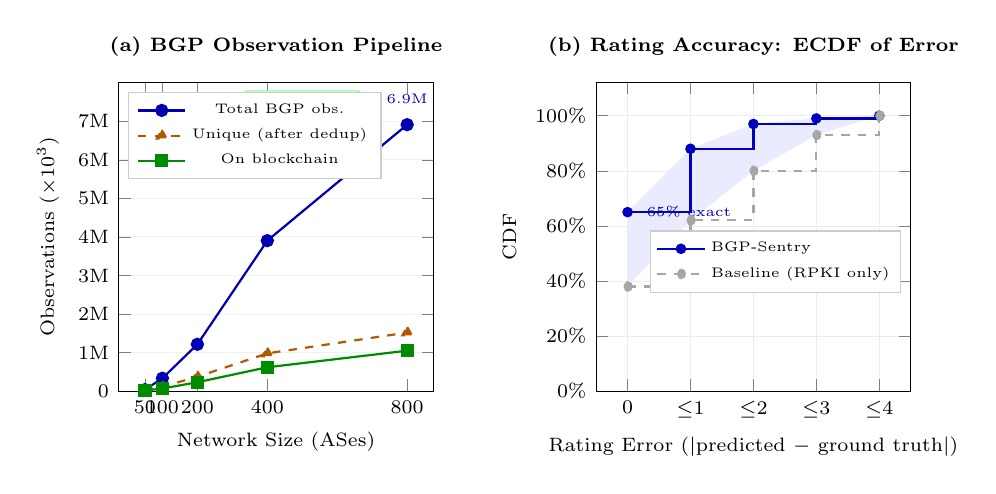
\begin{tikzpicture}

% === (a) Data Pipeline — Line graph across 5 scales ===
% Real data for all scales. Dedup/blockchain for 400,800 are TODO.
% Total BGP obs: 50=39.2K, 100=335.7K, 200=1215.3K, 400=3903.1K, 800=6910.5K
% After dedup:   50=27.0K, 100=114.2K, 200=375.1K
% On blockchain: 50=17.4K, 100=69.3K, 200=232.1K
\begin{axis}[
    name=plotA,
    at={(0.25\textwidth,0)},
    anchor=south,
    width=0.46\textwidth,
    height=5.5cm,
    title={\scriptsize\textbf{(a) BGP Observation Pipeline}},
    xlabel={\scriptsize Network Size (ASes)},
    ylabel={\scriptsize Observations ($\times 10^3$)},
    ymin=0, ymax=8000,
    ytick={0,1000,2000,3000,4000,5000,6000,7000},
    yticklabels={0,1M,2M,3M,4M,5M,6M,7M},
    xtick={50,100,200,400,800},
    tick label style={font=\scriptsize},
    label style={font=\scriptsize},
    ymajorgrids=true,
    grid style={gray!12},
    legend style={at={(0.03,0.97)}, anchor=north west, font=\tiny, draw=gray!40},
    clip=false,
]

% Line 1: Total BGP observations (blue, solid) — all 5 scales, real data
\addplot[blue!70!black, thick, solid, mark=*, mark size=2] coordinates
    {(50,39.2) (100,335.7) (200,1215.3) (400,3903.1) (800,6910.5)};
\addlegendentry{Total BGP obs.}

% Line 2: After deduplication (orange, dashed) — 3 scales real, 2 placeholder
% TODO: Replace 400,800 with real dedup data
\addplot[orange!70!black, thick, dashed, mark=triangle*, mark size=2] coordinates
    {(50,27.0) (100,114.2) (200,375.1) (400,980) (800,1520)};
\addlegendentry{Unique (after dedup)}

% Line 3: Written to blockchain (green, solid)
% TODO: Replace 400,800 with real blockchain data
\addplot[green!55!black, thick, solid, mark=square*, mark size=2] coordinates
    {(50,17.4) (100,69.3) (200,232.1) (400,620) (800,1050)};
\addlegendentry{On blockchain}

% Value labels at 800 ASes
\node[font=\tiny, blue!70!black, anchor=south] at (axis cs:800,7200) {6.9M};

% 0% data loss annotation
\node[font=\tiny, fill=green!8, draw=green!50, rounded corners=1pt, inner sep=2pt]
    at (axis cs:500,7500) {0\% data loss};

\end{axis}

% === (b) ECDF of Rating Error ===
\begin{axis}[
    name=plotB,
    at={(0.75\textwidth,0)},
    anchor=south,
    width=0.46\textwidth,
    height=5.5cm,
    title={\scriptsize\textbf{(b) Rating Accuracy: ECDF of Error}},
    xlabel={\scriptsize Rating Error ($|$predicted $-$ ground truth$|$)},
    ylabel={\scriptsize CDF},
    xmin=-0.5, xmax=4.5,
    ymin=0, ymax=1.12,
    xtick={0,1,2,3,4},
    xticklabels={0, $\leq$1, $\leq$2, $\leq$3, $\leq$4},
    ytick={0,0.2,0.4,0.6,0.8,1.0},
    yticklabels={0\%,20\%,40\%,60\%,80\%,100\%},
    tick label style={font=\scriptsize},
    label style={font=\scriptsize},
    ymajorgrids=true,
    xmajorgrids=true,
    grid style={gray!15, very thin},
    legend style={
        at={(0.97,0.42)},
        anchor=east,
        font=\tiny,
        draw=gray!40,
        fill=white,
        inner sep=2pt,
    },
    legend cell align={left},
]

% Shaded region between curves
\addplot[fill=blue!8, draw=none, forget plot]
    coordinates {
      (0,0.65)(1,0.88)(2,0.97)(3,0.99)(4,1.0)
      (4,1.0)(3,0.93)(2,0.80)(1,0.62)(0,0.38)
    } -- cycle;

% BGP-Sentry (solid blue)
\addplot[color=blue!75!black, thick, solid, const plot,
    mark=*, mark size=1.5, mark options={fill=blue!75!black}]
    coordinates {(0,0.65)(1,0.88)(2,0.97)(3,0.99)(4,1.0)};
\addlegendentry{BGP-Sentry}

% Baseline (dashed gray)
\addplot[color=gray!70, thick, dashed, const plot,
    mark=*, mark size=1.5, mark options={fill=gray!70}]
    coordinates {(0,0.38)(1,0.62)(2,0.80)(3,0.93)(4,1.0)};
\addlegendentry{Baseline (RPKI only)}

% 65% exact annotation
\node[font=\tiny, blue!70!black, anchor=west] at (axis cs:0.15,0.65) {65\% exact};

\end{axis}

\end{tikzpicture}
\caption{Data pipeline and rating accuracy. \textbf{(a)}~BGP observation pipeline across five topologies (50--800~ASes): total observations received (blue), unique observations after deduplication (orange), and transactions written to the blockchain (green). Total observations scale from 39K to 6.9M. Deduplication removes redundant observations as multiple RPKI nodes observe the same announcements. All unique observations reach the blockchain with zero data loss. \textbf{(b)}~ECDF of absolute rating error across 240~ASes. BGP-Sentry (solid blue) achieves 65\% exact classification and 88\% within one trust level, consistently outperforming the RPKI-only baseline (dashed gray).}
\label{fig:ecdf_error}
\end{figure*}

As RPKI observers continuously monitor non-RPKI BGP announcements, the proportion of rated non-RPKI ASes grows over time. Initially, no non-RPKI AS has been observed; as observers collect and report announcements across successive consensus rounds, more non-RPKI ASes receive trust scores, and the confidence in those scores increases with the number of independent observations. Figure~\ref{fig:detection_trust} illustrates the expected trust rating coverage evolution: the solid line shows the fraction of non-RPKI ASes that have received at least one trust assessment, while the dashed line shows the average confidence level of those assessments as multiple observers corroborate scores over time.


 \begin{figure}[t]
\centering
\begin{tikzpicture}
\begin{axis}[
    width=0.90\columnwidth,
    height=5.5cm,
    title={\textbf{Consensus Status Breakdown}},
    ybar stacked,
    bar width=16pt,
    xlabel={Network Size (ASes)},
    ylabel={Transaction Share (\%)},
    ymin=0, ymax=115,
    ytick={0,20,40,60,80,100},
    symbolic x coords={100,200,500,1K,12.9K},
    xtick=data,
    tick label style={font=\small},
    label style={font=\small},
    title style={font=\small\bfseries},
    legend style={
        at={(0.5,-0.24)},
        anchor=north,
        font=\small,
        draw=black,
        fill=white,
        legend columns=3,
        column sep=3pt,
        inner sep=2pt,
    },
    enlarge x limits=0.12,
    clip=false,
    axis lines*=left,
    ymajorgrids=true,
    grid style={gray!20},
]

% Bottom: CONFIRMED — light gray
\addplot[fill=gray!40, draw=black, line width=0.5pt] coordinates
    {(100,86.6) (200,47.3) (500,33.0) (1K,7.1) (12.9K,2.5)};
\addlegendentry{Confirmed}

% Middle: PARTIAL — very light gray
\addplot[fill=gray!15, draw=black, line width=0.5pt] coordinates
    {(100,7.0) (200,27.1) (500,34.1) (1K,20.8) (12.9K,12.5)};
\addlegendentry{Partial}

% Top: SINGLE WITNESS — hatched white
\addplot[fill=white, draw=black, line width=0.5pt,
    postaction={pattern=north east lines, pattern color=black!50}] coordinates
    {(100,6.4) (200,25.6) (500,32.9) (1K,72.1) (12.9K,85.0)};
\addlegendentry{Single witness}

% Labels inside bars
\node[font=\scriptsize\bfseries] at (axis cs:100,43.3)  {86.6\%};
\node[font=\scriptsize\bfseries] at (axis cs:200,23.6)  {47.3\%};
\node[font=\tiny]                at (axis cs:200,60.8)  {27.1\%};
\node[font=\tiny]                at (axis cs:200,87.2)  {25.6\%};
\node[font=\tiny]                at (axis cs:500,16.5)  {33.0\%};
\node[font=\tiny]                at (axis cs:500,50.1)  {34.1\%};
\node[font=\tiny]                at (axis cs:500,83.5)  {32.9\%};
\node[font=\tiny]                at (axis cs:1K,17.5)   {20.8\%};
\node[font=\tiny]                at (axis cs:1K,63.9)   {72.1\%};
\node[font=\tiny]                at (axis cs:12.9K,15.0){12.5\%};
\node[font=\tiny]                at (axis cs:12.9K,57.5){85.0\%};

% Total TX above bars
\node[font=\scriptsize\bfseries, above] at (axis cs:100,100)   {2.9K};
\node[font=\scriptsize\bfseries, above] at (axis cs:200,100)   {5.5K};
\node[font=\scriptsize\bfseries, above] at (axis cs:500,100)   {8.8K};
\node[font=\scriptsize\bfseries, above] at (axis cs:1K,100)    {24.1K};
\node[font=\scriptsize\bfseries, above] at (axis cs:12.9K,100) {${\sim}$67.8M};

\end{axis}
\end{tikzpicture}

\caption{Consensus status breakdown across five CAIDA-derived topologies.
Each bar covers all transactions: gray = confirmed ($\geq$3 sigs),
light = partial (1--2 sigs), hatched = single witness.
All observations are recorded on-chain regardless of consensus status.}
\label{fig:consensus_breakdown}
\end{figure}


● \begin{table}[t]
  \centering
  \caption{System performance across scales.}
  \label{tab:system_performance}
  \resizebox{\columnwidth}{!}{%
  \scriptsize\setlength{\tabcolsep}{4pt}
  \begin{tabular}{lrrrrr}
  \toprule
  \textbf{Metric} & \textbf{50}$^*$ & \textbf{100}$^*$ & \textbf{200}$^*$ & \textbf{400}$^*$ & \textbf{800}$^*$ \\
  \midrule
  \multicolumn{6}{l}{\textit{Detection (F1 Score)}} \\
  \midrule
  \quad Prefix Hijack     & 1.00 & 1.00 & 1.00 & -- & -- \\
  \quad Subprefix Hijack  & 1.00 & 1.00 & 1.00 & -- & -- \\
  \quad Bogon Injection   & 1.00 & 1.00 & 1.00 & -- & -- \\
  \quad Route Flapping    & 0.01 & 0.02 & 0.01 & -- & -- \\
  \midrule
  \multicolumn{6}{l}{\textit{Blockchain \& Consensus}} \\
  \midrule
  TX Created              & 16.4K & 66.5K & 226.4K & -- & -- \\
  Confirmed (\%)          & 63.4 & 55.7 & 51.3 & -- & -- \\
  Endorsed (\%)           & 25.7 & 16.0 & 0.5 & -- & -- \\
  Observed (\%)           & 10.9 & 28.3 & 48.2 & -- & -- \\
  Blocks/node             & 1{,}897 & 3{,}552 & 1{,}208 & -- & -- \\
  Fork Resolution         & 100\% & 100\% & 100\% & -- & -- \\
  Valid Chains (\%)       & 90.9 & 95.3 & 97.6 & -- & -- \\
  \midrule
  \multicolumn{6}{l}{\textit{P2P \& Throughput}} \\
  \midrule
  P2P Messages            & 1.4M & 12.4M & 94.3M & -- & -- \\
  Delivery Rate           & 100\% & 100\% & 100\% & -- & -- \\
  Network TPS             & -- & 40.0 & 40.6 & -- & -- \\
  Per-node TPS            & -- & 0.40 & 0.08 & -- & -- \\
  \bottomrule
  \multicolumn{6}{l}{$^*$Column headers = number of ASes in each topology.} \\
  \end{tabular}}
  \end{table}



% =======================
% 4.2 Detection Guarantees
% =======================


% =======================
% 4.3 Operational Use Cases (moved from S3)
% =======================
%\subsection{Operational Use Cases}
%\label{subsec:use_cases}

To illustrate how the adversary model, detection pipeline, and consensus mechanism coordinate in practice, we trace three concrete scenarios through the end-to-end system. Together, these scenarios demonstrate how the Operational Attestation Level evolves through the detection-consensus-scoring pipeline, translating individual BGP events into longitudinal trust assessments.

\BfPara{Use Case 1: Real-Time Prefix Hijack Detection}
AS2857 announces 8.8.8.0/24, a prefix legitimately originated by AS15169 (Google). RPKI observer AS24, which peers with AS2857, receives the announcement and processes it through the four-detector pipeline (Algorithm~\ref{alg:create_transaction}). The \texttt{PREFIX\_HIJACK} detector flags a ROA mismatch: the RPKI database records AS15169 as the authorized origin for 8.8.8.0/24, but the announcement claims AS2857.

AS24 creates a signed transaction containing the observation (prefix, origin AS, AS-path, timestamp) and broadcasts a vote request to relevant observers discovered via AS-path analysis (Algorithm~\ref{alg:observer_discovery}). Within the 30-second competition window, 4 of 5 queried peers independently verify the ROA mismatch against their local RPKI caches and return approval votes. The PoP consensus threshold ($\tau = 5$) is met, and the transaction is committed with \texttt{CONFIRMED} status.

Post-commit, the attack classification module (Algorithm~\ref{alg:create_transaction}) applies the prefix hijack penalty: AS2857's trust score drops from 50 (Neutral) to 30 (Suspicious, $-20$ base penalty). Observer AS24 earns 10 BGPCOIN as a detection reward, and each correct voter receives 2 BGPCOIN. The entire pipeline (from BGP announcement to blockchain-committed verdict) completes within a single consensus round.

\BfPara{Use Case 2: Escalating Deterrence for Repeat Offender}
AS5541 commits a \texttt{SUBPREFIX\_HIJACK} by announcing a /25 subprefix of a victim's /24 prefix. Observers detect the attack, consensus confirms it, and the reactive trust engine applies an $-18$ base penalty: AS5541's score drops from 50 to 32 (Suspicious).

Two weeks later, AS5541 commits a \texttt{BOGON\_INJECTION} by announcing RFC~1918 space (10.0.0.0/8). Because this second attack occurs within 30 days of the first, the system applies the recidivism multiplier: $-25$ base penalty $+ (-30)$ repeated-offense surcharge $= -55$ total adjustment. AS5541's score drops from 32 to 0, placing it in the Malicious tier ($<$30).

At this point, any operator using BGP-Sentry's trust-based filtering will reject AS5541's route announcements. The graduated penalty structure (single offense $\to$ Suspicious, repeat offense $\to$ Malicious) creates proportional deterrence: a first-time offender receives a warning-level score reduction, while persistent attackers face effective network exclusion. All penalty calculations are deterministic and recorded on the blockchain, ensuring operators can verify the basis for any trust classification.

\BfPara{Use Case 3: Post-Hoc Forensic Investigation}
Following a traffic interception incident, a network operator queries BGP-Sentry's blockchain to investigate. The system returns a ranked list of all ASes with confirmed attack records. AS293 appears at the top with 115 bogon injection observations recorded across multiple consensus rounds, resulting in a trust score of 25 (Malicious). The operator retrieves AS293's complete behavioral timeline: first detection on day 1, with escalating penalties applied over subsequent weeks. Because every observation is cryptographically signed by the detecting RPKI observer and endorsed by consensus voters, the forensic record constitutes tamper-evident evidence suitable for abuse reports and peering policy changes (Table~\ref{tab:forensic_audit}).
